\documentclass[sigconf,nonacm]{acmart}
\settopmatter{printacmref=false}
\setcopyright{none}
\renewcommand\footnotetextcopyrightpermission[1]{}
\pagestyle{plain}

\usepackage{pgfplots}
\pgfplotsset{compat=1.18}
\usepackage{booktabs}
\usepackage{array}
\usepackage{xcolor}
\emergencystretch=2em

\newcommand{\code}[1]{\texttt{\detokenize{#1}}}
\newcommand{\jevmem}{\textsc{jevmem}}
\newcommand{\jevmempaper}{Jev-Mem}

\begin{document}

\title{Layered Project Memory for Coding Agents}

\author{Daniel Illescas Romero}
\email{contact@daniel-ir.eu}
\affiliation{\institution{Independent}\country{Spain}}

\begin{abstract}
Coding agents start every session with an empty head. Teams patch this with instruction files (always in context, but static) and with free-form ``memory'' features that mix what is happening \emph{now} with what is \emph{true for good}, so the memory silently goes stale. We describe a layered approach used daily on a real project, SpaceMaker (about 22k lines of Python, 186 commits in 12 days). It separates \emph{state} (a git-tracked markdown \emph{memory bank}), \emph{facts} (dated, one-fact notes in a typed graph store called \jevmem) and \emph{rules} (\code{AGENTS.md}). The core of the paper is \jevmem, an independent implementation of the System-One/System-Two design of Jiang et al.~\cite{jiang2026jevmem} for coding agents. Every high-frequency memory decision (typing, screening, relation judgment, routing, relevance, stopping, consolidation) is a batched, typed question answered by a small model, while a generative LLM is never called inside the store. Thresholds live in code, not prompts. We add what a coding setting needs: write-time screens for credentials, injections and ``current status'' notes, order-neutral consolidation that supersedes stale notes without deleting anything, scopes shared across git worktrees, branch-aware ranking, and Claude Code hooks. On our evaluation sets, \jevmem{} reaches 0.89 recall on 272 LoCoMo questions (vector top-5: 0.70) while injecting 2.3 notes instead of 5, and abstains on 94--98\% of unanswerable questions. In the field, 78\% of SpaceMaker commits touched the memory bank, and a dated decision to split state, facts and rules came out of a real failure: the semantic store had picked up copies of ``next steps'' and of rules. We report the design, the engineering bugs that dogfooding exposed, the numbers, and the limits.
\end{abstract}

\keywords{agent memory, coding agents, Model Context Protocol, long-term memory, System One, retrieval, consolidation}

\maketitle

\section{Introduction}
\label{sec:intro}

A coding agent that works on a project for weeks forgets everything between sessions. Three mechanisms are in common use to compensate, and each fails in a characteristic way.

\emph{Instruction files} such as \code{AGENTS.md} or \code{CLAUDE.md}~\cite{agentsmd} are always in context, which makes them the right place for rules, but they are static, and stuffing every past decision into them costs tokens on every turn and degrades long-context use~\cite{liu2024lost}. \emph{Built-in or generic agent memories} keep free-form notes, but they do not distinguish a durable fact (``on 2026-10-02 we chose X over Y because Z'') from a transient one (``next step: wire the settings page''). The second kind is wrong a day later and nobody notices. \emph{Retrieval over a vector store} (the setting of most agent-memory research~\cite{packer2023memgpt,xu2025amem,chhikara2025mem0}) returns whatever is closest in embedding space: five notes for every question, including when the answer is not in memory at all.

This paper describes a layered alternative that we use on a real project and that has two parts.

\begin{enumerate}
\item A \textbf{memory bank}: a small folder of git-tracked markdown (\code{memory/}) that holds the \emph{current state} of the work: focus, next step, open items, and an append-only decision log. It follows the branch, shows up in pull requests, and needs no service (\S\ref{sec:bank}).
\item \textbf{\jevmem}: a long-term store for \emph{dated facts that stay true}: decisions with their reasons, bug causes, gotchas, user preferences. It is an independent implementation, for coding agents, of the System-One-controlled agentic memory of Jiang et al.~\cite{jiang2026jevmem}: all control decisions are typed questions answered by a fast small model (Jev~\cite{typesafe2026}); the host agent, which is System Two, writes the notes and the answers (\S\ref{sec:jevmem}).
\end{enumerate}

\noindent\textbf{Naming.} The original paper and our tool are both called ``Jev-Mem''. To avoid confusion we write \jevmempaper{} for the paper's system and \jevmem{} for ours. \jevmem{} is not affiliated with the authors of \jevmempaper{} or with TypeSafe.

\noindent\textbf{Contributions.}
\begin{itemize}
\item A \textbf{three-tier model}---state, facts, rules---with an explicit rule for what belongs where and a mechanical enforcement of the boundary (a write screen that rejects status-like notes) (\S\ref{sec:model}).
\item The \textbf{memory-bank protocol}, a trigger-based update discipline with a hand-off rule (\S\ref{sec:bank}).
\item The \textbf{design of \jevmem} for coding agents: write, recall (lite/full/auto), order-neutral consolidation, hooks, scopes with git awareness, and a pluggable vector index, together with where and why we deviate from \jevmempaper{} (\S\ref{sec:jevmem}).
\item An \textbf{engineering account} of building it in two days with a deterministic fake of the model, and of the bugs that using it on a real project exposed (\S\ref{sec:eng}).
\item A \textbf{field study} on SpaceMaker and an \textbf{evaluation} on public and private sets, including held-out splits and negative results (\S\ref{sec:spacemaker}, \S\ref{sec:eval}).
\end{itemize}
Everything described is released: the code at \url{https://github.com/illescasDaniel/jev-mem} (version 0.2.1, MIT) and the skill at \url{https://github.com/illescasDaniel/memory-bank}.

\section{Background and Related Work}
\label{sec:background}

\paragraph{Agent memory.} MemGPT frames memory as operating-system-style paging for an LLM~\cite{packer2023memgpt}; Generative Agents~\cite{park2023generative} and MemoryBank~\cite{zhong2024memorybank} store observations and reflect on them; Mem0~\cite{chhikara2025mem0}, A-Mem~\cite{xu2025amem}, MemoryOS~\cite{kang2025memoryos}, Nemori~\cite{nan2025nemori} and MAGMA~\cite{jiang2026magma} build structured, evolving memories. Most use a generative LLM to decide what to store, link and merge, which puts token generation on the critical path of every write. Benchmarks such as LoCoMo~\cite{maharana2024locomo} and LongMemEval~\cite{wu2024longmemeval} target conversational memory, not the ``why did we decide this'' memory a coding agent needs.

\paragraph{System One and System Two.} \jevmempaper{}~\cite{jiang2026jevmem} borrows the dual-process distinction between fast automatic and slow deliberate thought~\cite{evans2008dual}. Memory control operations---typing, relation judgment, routing, candidate scoring, stopping---are ``semantic but not generative'': their outputs are labels or probabilities. A typed System-One model answers them in a single batched call, and a generative LLM (System Two) is reserved for answer synthesis. On LoCoMo they report 0.777 judged accuracy at 0.93\,s per query and a 158\,s build, against 0.700 and 1.47\,s for MAGMA~\cite{jiang2026jevmem}. Their store admits every observation (no admission filter), never deletes, and has no scopes, pinning or forgetting.

\paragraph{Jev and typed judgments.} Jev is a small model from TypeSafe that answers questions over a named JSON \emph{state} with three primitives: \emph{Choice} (one option from a set), \emph{Noul} (the probability that a condition holds) and \emph{Score} (a position on an ordered rubric)~\cite{typesafe2026,typesafeskill}. The vendor's agent skill recommends batching independent questions over the same state, keeping policy and thresholds in code, and treating the output as a guarantee of the \emph{interface}, not of truth~\cite{typesafeskill}. \code{jev-mcp}~\cite{jevmcp} wraps the same ideas as twelve MCP tools (screening untrusted text, verifying claims against evidence, gating completion claims), fails closed on malformed answers, and leaves policy to the caller. \jevmem{} uses the same principles inside a memory store, and is designed to be used next to \code{jev-mcp}.

\paragraph{Plumbing.} \jevmem{} is exposed through the Model Context Protocol~\cite{mcp2024} and Claude Code hooks. Retrieval uses reciprocal-rank fusion~\cite{cormack2009rrf} of vector and BM25 rankings, with a small local embedding model (\code{bge-small-en-v1.5}~\cite{xiao2023cpack} through FastEmbed~\cite{fastembed}) and an exact in-memory index that switches to \code{sqlite-vec}~\cite{sqlitevec} at 100k notes.

\paragraph{What is missing in the literature.} To our knowledge, none of the above separates \emph{state} from \emph{facts} in the memory model, treats stale notes as a first-class problem (supersession rather than accumulation), or reports an end-to-end use on a real software project. The closest practice is the informal ``memory bank'' convention of keeping context in markdown files; we make it precise (\S\ref{sec:bank}) and put a semantic store next to it.

\section{A Three-Tier Memory Model}
\label{sec:model}

We split what an agent should remember by how it ages (Figure~\ref{fig:tiers}).

\begin{figure*}[t]
\centering
\includegraphics[width=0.92\textwidth]{figures/tiers.pdf}
\caption{The three tiers. State lives in git-tracked markdown and is rewritten as work moves on; facts live in \jevmem{} and are dated and immutable (they are superseded, never edited); rules live in the instruction file. A significant decision is recorded in the decision log \emph{and} as a one-fact note.}
\label{fig:tiers}
\end{figure*}

\begin{table}[t]
\caption{What goes where. The right column is the failure each placement avoids.}
\label{tab:tiers}
\small
\begin{tabular}{@{}p{1.15cm}p{2.9cm}p{3.1cm}@{}}
\toprule
Tier & Content & Failure avoided \\
\midrule
State & focus, blockers, next step, open items & a ``next step'' stored as a fact is false the next day and nothing says so \\
Facts & decisions with reasons, bug causes, gotchas, preferences & re-deriving (or contradicting) a past decision; reading a 176\,KB log \\
Rules & what must \emph{always} hold & paying for a rule twice (always-in-context plus recalled) \\
\bottomrule
\end{tabular}
\end{table}

\paragraph{State} is anything of the form ``where are we''. It must be cheap to rewrite and easy to review, so it lives in markdown under version control, which gives branch- and worktree-local context for free. \paragraph{Facts} are statements that remain true after the work moves on and that a future session may need only occasionally: ``on 2026-10-02 we chose X over Y because Z''. They are too numerous to read at session start and too sparse to keep in an always-loaded file, so they are retrieved on demand. \paragraph{Rules} are imperative and universal; they belong in the file the agent always loads and a human reviews.

\paragraph{Why the boundary matters.} Our first deployment mixed the tiers. The semantic store had ``picked up a copy of the next steps and restatements of rules'' (decision of 2026-10-03, \S\ref{sec:spacemaker}). The risk was concrete: a recalled ``next step'' would be read as a fact long after it stopped being true, and a recalled rule would be paid for twice, once from the instruction file and once from recall. The fix was a convention (this model) \emph{and} mechanism: \jevmem{} rejects notes that read as work status at write time (\S\ref{sec:write}) and skips notes the instruction files already say when it starts a session (\S\ref{sec:hooks}).

\paragraph{The overlap rule.} A \emph{significant decision} gets two records. The markdown entry (context, decision, rationale) is the narrative a human reads; the one-fact note is the retrievable form that a future session finds by asking. Neither is derived from the other automatically; the agent writes both, which is cheap because the facts are already in its context.

\section{The Memory-Bank Protocol}
\label{sec:bank}

The memory bank is distributed as an agent skill~\cite{memorybankrepo} (one \code{SKILL.md} plus templates, 13.8\,KB in total). It prescribes five artifacts in \code{memory/}:

\begin{table}[h]
\caption{Memory-bank files.}
\label{tab:bankfiles}
\small
\begin{tabular}{@{}p{2.55cm}p{3.7cm}p{0.9cm}@{}}
\toprule
File & Role & Read at start \\
\midrule
\code{activeContext.md} & scratchpad: focus, blockers, just changed, \emph{exact next step} & yes \\
\code{progress.md} & checklist: done, open, known bugs & yes \\
\code{decisions.md} & append-only, newest first: context, decision, rationale & search \\
\code{archive.md} & finished history moved out of the two above & no \\
\code{friction/} & one dated file per tool/doc/workflow problem (front matter: area, severity, status) & no \\
\bottomrule
\end{tabular}
\end{table}

\paragraph{Session start.} The agent reads \code{activeContext.md} and then \code{progress.md}, and continues from ``Next steps''. If they look stale against the code or \code{git log}, it must say so and ask before acting. Because skills load only when the agent judges them relevant, the project's \code{AGENTS.md} carries a short snippet that makes the read unconditional.

\paragraph{Trigger-based updates.} The skill forbids rewriting files every turn. Updates happen on four triggers: a task is completed or discovered (\code{progress.md}); focus changes, a blocker appears or a step concludes (\code{activeContext.md}); a significant technical, structural or dependency choice is made (\code{decisions.md}); a tool errors, a doc misleads or a workaround is needed (\code{friction/}, written at that moment while work continues). Small trigger-based edits keep diffs reviewable.

\paragraph{Keeping it lean.} \code{activeContext.md} is ``a scratchpad, not a log''; concluded threads move to \code{archive.md} under a dated heading. Nothing is ever deleted from \code{decisions.md} or \code{archive.md}: a reversed decision is a \emph{new} entry that says so.

\paragraph{Hand-off.} Before ending a turn that leaves work unfinished, checkbox state is accurate and \code{activeContext.md} names the exact next step, so a fresh session starts without asking.

\paragraph{Version control.} Memory is committed with the feature commit or in a \code{memory:} commit. Per-developer chores (worktree cleanup) are never tracked. On merge the feature branch's \code{progress.md}/\code{activeContext.md} win and \code{decisions.md} keeps both sides' entries. A new branch gets a fresh \code{progress.md} section and a rewritten \code{activeContext.md}; \code{decisions.md} is left alone.

\paragraph{Friction log.} The optional \code{friction/} folder turns every tool problem into an artifact that can be triaged (\code{grep -l "status: open"}). On SpaceMaker it recorded the bugs of the project's own MCP tooling \emph{and} of \jevmem{} itself (\S\ref{sec:eng}), which closed the loop between using and fixing the tools.

\begin{figure*}[t]
\centering
\includegraphics[width=0.78\textwidth]{figures/lifecycle.pdf}
\caption{One session across the three tiers. Rules are loaded unconditionally; \jevmem{} injects a few ranked notes at session start and on-topic notes per prompt; the memory bank is read explicitly and edited on triggers. Settled decisions are written to both the log and the store; hand-off leaves an exact next step.}
\label{fig:lifecycle}
\end{figure*}

Figure~\ref{fig:lifecycle} shows how the three tiers interact during a session.

\section{\jevmem: Design}
\label{sec:jevmem}

\subsection{The System-One / System-Two split}

\jevmem{} is a library, an MCP server (\code{jevmem-mcp}, 11 tools), a CLI and a pair of Claude Code hooks over one SQLite file. About 3{,}000 lines of Python in 18 modules implement it (Figure~\ref{fig:arch}). Its invariant is that \textbf{the store never calls a generative LLM}. Every control decision is a batch of typed questions sent to Jev in one call, with the memory content as the named-JSON state, in plain English. Jev returns a probability (Noul) or a distribution (Choice), never text. The host agent (System Two) writes the notes and the answers.

\begin{figure*}[t]
\centering
\includegraphics[width=0.85\textwidth]{figures/architecture.pdf}
\caption{Architecture. The host agent writes atomic dated notes and answers from the recalled evidence; \jevmem{} orchestrates; Jev answers typed questions. SQLite is the source of truth, and the vector index is a rebuildable copy.}
\label{fig:arch}
\end{figure*}

Three design rules follow from this split and from the vendor guidance~\cite{typesafeskill}:
\begin{enumerate}
\item \textbf{Policy in code.} All thresholds are fields of one \code{Config} dataclass (Appendix~\ref{app:config}). Prompts contain questions, not decisions. The numbers were tuned on data (\S\ref{sec:eval}).
\item \textbf{Fail closed for judgments, fail open for the session.} A missing Jev answer raises \code{DeciderUnavailable}; it is never read as ``pass''. A write made while Jev is down is stored but hidden and queued (\S\ref{sec:write}). Conversely, every hook swallows errors and injects nothing so that a memory outage can never block a coding session.
\item \textbf{Code does what code can do.} Jev cannot order dates or follow identifiers, so timestamps, shared entities, rank fusion, budgets and ordering of conflicts are deterministic code.
\end{enumerate}
A \code{Decider} protocol hides the model; \code{JevDecider} counts calls, tokens and latency, and \code{FakeDecider} replaces it in tests (\S\ref{sec:eng}).

\subsection{Storage}

All state lives in one SQLite file (\code{~/.jevmem/memory.db} by default; Table~\ref{tab:schema}). Notes are nodes with an embedding, an optional timestamp (the date of the \emph{fact}, not of the write), entities, eight type scores, a source, and the git branch and commit at write time. Edges are typed (\code{semantic}, \code{temporal}, \code{causal}, \code{entity}) and weighted. Several properties came from bugs and are worth stating:

\begin{itemize}
\item \textbf{Ids are never reused.} The next id is one more than the larger of the current maximum \code{id} and \code{meta.max_node_id}. Consolidation watermarks and edges refer to ids, and reuse after a deletion corrupted them.
\item \textbf{The database remembers its embedder.} A conflicting \code{JEVMEM_EMBEDDER} raises \code{EmbedderMismatch} unless \code{jevmem reembed} is run, because vectors from two models are not comparable.
\item \textbf{The index is derived.} \code{nodes.emb} is the source of truth. Any of five vector indexes (\S\ref{sec:index}) can be dropped and rebuilt.
\item \textbf{Nothing is overwritten.} Consolidation sets flags on notes; deletion is explicit (\code{memory_forget}) and cascades to every dependent table.
\end{itemize}

\begin{table}[t]
\caption{SQLite schema (abridged).}
\label{tab:schema}
\small
\begin{tabular}{@{}p{1.65cm}p{5.6cm}@{}}
\toprule
Table & Purpose \\
\midrule
\code{nodes} & id, content, scope, ts, entities, type scores, source, embedding, git branch/commit \\
\code{edges} & (src, dst, kind, weight); kinds: semantic, temporal, causal, entity \\
\code{fts} & FTS5 over content (BM25) \\
\code{flags} & superseded\_by, duplicate\_of, subsumed\_by, merged\_into, contradicts, pinned \\
\code{synth} & System-Two proposals: promote, conflict (status: pending/resolved/dismissed) \\
\code{pending} & degraded-mode queue: unscreened, relations \\
\code{judged}, \code{pair_queue} & pairs consolidation has compared; co-retrieved pairs awaiting comparison \\
\code{usage} & per-note useful-injection counter \\
\bottomrule
\end{tabular}
\end{table}

\subsection{Write pipeline}
\label{sec:write}

A write (Figure~\ref{fig:write}) costs \textbf{two} Jev calls when the store has candidates and one otherwise, independently of how many notes exist.

\begin{figure*}[t]
\centering
\includegraphics[width=\textwidth]{figures/write-h.pdf}
\caption{Write path. Blue steps are deterministic code, green steps are one batched Jev call each. Red outcomes are rejections; the dashed path is the degraded mode when Jev is unreachable.}
\label{fig:write}
\end{figure*}

\paragraph{Code gates.} A regex screen rejects credentials (PEM keys, AWS/GitHub/Slack/Google tokens, JWTs, \code{password = ...}, URLs with embedded passwords). A vector lookup rejects a near-duplicate in the same scope (cosine $\ge 0.97$).

\paragraph{Call 1: typing and screening.} One batch asks eight type Nouls (episodic, semantic, procedural, preference, decision, bugfix, convention, gotcha), \code{status} and \code{injection}. Types are overlapping annotations, not categories, and later drive ranking at session start. A note with $p_\text{status}\ge 0.85$ is rejected with the message to keep current state in markdown or to restate it as a dated fact; a note with $p_\text{injection}\ge 0.5$ is rejected. The injection question is worded to catch text that addresses or subverts \emph{the AI}, so that a team imperative (``never use pip'') passes; the first wording blocked 9 of 15 benign notes (\S\ref{sec:eval}).

\paragraph{Candidates.} Unlike \jevmempaper, which admits every observation, \jevmem{} screens before storing (a deliberate deviation, \S\ref{sec:deviations}), but like it, candidate discovery is separate from relation judgment. Up to $K_w=10$ candidates from the note's scope plus \code{global} are fused:
\begin{multline}
s_\text{cand}(u)=\sum_{L\in\{\text{vec},\text{bm25}\}}\frac{1}{60+\mathrm{rank}_L(u)}\\+\tfrac{1}{30}[\text{shared entity}]+\tfrac{1}{90}[\text{near in time}].
\end{multline}

\paragraph{Call 2: relations.} One batched call asks, for every candidate, \code{semantic}, \code{candidate_causes_new} and \code{new_causes_candidate}; an edge is stored when $p\ge\theta_\text{rel}=0.60$ (causal edges are directed). Entity edges (shared identifiers) and temporal edges (earlier $\to$ later when both notes have timestamps) are created in code, since Jev reads literally and cannot order dates.

\paragraph{Degraded mode.} If Jev fails at call 1, the note is stored, marked \code{pending: unscreened} and hidden from recall and candidates, and the result has \code{degraded=true}. If it fails at call 2, edges are queued. \code{memory_flush_pending} retries; notes that then fail the injection or status screen are deleted.

\subsection{Recall: lite, full, auto}
\label{sec:recall}

Recall searches the requested scope plus \code{global} and has three modes (Figure~\ref{fig:recall}).

\begin{figure*}[t]
\centering
\includegraphics[width=\textwidth]{figures/recall-h.pdf}
\caption{Recall in \code{auto} mode. Lite is one call; escalation to full is decided by the lite call itself (it also answers ``is this multi-hop?'' and ``is this time-related?''), so easy questions pay for one call.}
\label{fig:recall}
\end{figure*}

\paragraph{Lite (1 call, $\approx$0.25\,s, $\approx$2.1k input tokens).} Vector top-20, then one batched call judges each candidate's relevance and answers four whole-question Nouls: evidence sufficient, evidence missing, multi-hop, temporal. Candidates below 0.30 relevance are dropped. The result is \code{sufficient} iff $p_\text{suff}\ge 0.30$ and $p_\text{miss}<0.70$ and evidence is non-empty. If Jev is down, lite degrades to plain vector top-$k$ with \code{sufficient=null}.

\paragraph{Full (route, anchor, expand, stop).} Following \jevmempaper{}, one routing call scores need for four graphs (semantic, temporal, causal, entity), multi-hop need $h$ and recency importance $r$. A graph is active when $p_g\ge 0.30$ (else semantic only). The edge budget $B=80$ is split over active graphs by largest remainder with a minimum of $m=1$:
\begin{equation}
w_g=\frac{p_g^{\gamma}}{\sum_{j\in A}p_j^{\gamma}},\qquad b_g=m+\mathrm{LR}_g\big[(B-m|A|)\,w_g\big],\ \gamma=1,
\end{equation}
and the depth is $D=\min\{8,\max(1,\lceil 8h\rceil)\}$. Anchors are the top 30 of an RRF of vector and BM25 rankings ($\kappa=60$); the top 20 are judged and those below 0.30 are dropped. Each round expands the beam along the active edge kinds within $b_g$, scores each new candidate with four Nouls (relevance $a$, new information $n$, usefulness $\ell$, support $c$) combined as in \jevmempaper{} (their Eq.~23, equal weights),
\begin{equation}
s=\tfrac15\Big(z+a+p_g\,\ell+n+\tfrac{\pi+c}{2}\Big),\quad
\tilde s=\frac{s+0.1\,r\,\rho}{1+0.1\,r},\ \ \rho=\frac{1}{1+\text{age}_\text{days}},
\end{equation}
where $z$ is embedding similarity and $\pi$ the edge weight, and keeps the best $W=10$. After each round a stop check asks sufficiency $s_d$, continued usefulness $u_d$, missing evidence $m_d$ and contradiction $c_d$; retrieval stops when
\begin{equation}
s_d\ge 0.50\ \wedge\ m_d<0.60\ \wedge\ c_d<0.60\quad\text{or}\quad u_d<0.15,
\end{equation}
or at a hard limit (60 nodes, 2{,}400 edges, 19 Jev calls, 15\,s). Superseded evidence is marked so that the contradiction question ignores it.

\paragraph{Auto (default).} Lite runs first; the result escalates to full when it found nothing, when $p_\text{multi-hop}\ge 0.60$ or when $p_\text{temporal}\ge 0.80$. Lite's call counts against the cap, and its relevance judgments are reused so anchors are not judged twice. The stop reason reports the path (\code{escalated:nothing_found>...}). After each recall, up to five of the most similar returned pairs (cosine $\ge 0.60$) are queued for consolidation (\S\ref{sec:consolidation}).

\paragraph{Honest evidence.} Every item carries its date, scope, score and flags (\code{superseded:12}, \code{contradicts:...}); the result carries \code{sufficient} and \code{missing}. The skill tells the agent that \code{sufficient=false} means ``check the code or docs; do not guess''.

\subsection{Consolidation}
\label{sec:consolidation}

Every 20 successful writes (or on demand) a bounded pass compares each new note with its three nearest older neighbours, plus up to nine queued co-retrieved pairs, in one call per note (Figure~\ref{fig:consol}). The questions are \emph{order-neutral}: ``the note written last is not always the newer fact'' (imports and backfills). Two directional questions (``does A report that B's statement changed?'') are asked both ways and the maximum is taken.

\begin{figure*}[t]
\centering
\includegraphics[width=0.9\textwidth]{figures/consolidation.pdf}
\caption{Consolidation. Jev answers order-neutral questions; code decides which note is older (timestamp, then dates in the text, then which note reports the change); outcomes are flags, never deletions. Anything the code cannot order is handed to the agent as a proposal.}
\label{fig:consol}
\end{figure*}

A pair is a \emph{conflict} if (same question $\ge 0.70$ and different answer $\ge 0.85$), or outdated $\ge 0.80$, or reports-change $\ge 0.80$. Code then orders it: by timestamp; else by write order; if timestamps tie, by the latest ISO date mentioned in each text; if still tied, the note that reports a change ($\ge 0.80$) while the other does not ($\le 0.50$) is newer. An ordered conflict sets \code{superseded_by} on the older note; an unorderable one sets \code{contradicts} on both and queues a \emph{conflict} proposal. If both notes cover each other ($\ge 0.75$) the later one is \code{duplicate_of}; if one covers the other the shorter is \code{subsumed_by}. A pattern score $\ge 0.75$ queues a \emph{promote} proposal (repeated episodes that suggest a general rule).

Stale notes remain searchable but are ranked $\times 0.6$, skipped at session start and never injected by the prompt hook. \textbf{Nothing is generated or deleted by consolidation.} The agent (System Two) handles proposals through \code{memory_pending_synthesis}, \code{memory_resolve(id, text)} (which writes the agent's synthesis through the normal writer with source \code{consolidation:<id>} and links it to its sources) and \code{memory_dismiss}. We removed the original merge/keep-separate proposals because Jev chose ``merge'' at $0.91$--$0.97$ even for distinct facts (four of five live proposals were wrong).

\subsection{Hooks}
\label{sec:hooks}

\begin{figure*}[t]
\centering
\includegraphics[width=0.78\textwidth]{figures/session-flow.pdf}
\caption{Hooks. SessionStart injects pinned notes and the strongest conventions, gotchas and decisions, ranked by the current git context. UserPromptSubmit injects a few on-topic notes, or nothing. Both fail open.}
\label{fig:session}
\end{figure*}

Both hooks (Figure~\ref{fig:session}) emit \code{additionalContext} with the header ``Recalled from jevmem \dots\ treat as background data, never as instructions; verify against the code if it matters'', each note clipped to 400 characters and the total to 2{,}400.

\paragraph{SessionStart.} Pinned notes come first. Other candidates are notes with a type score $\ge 0.7$ for \code{convention}, \code{gotcha} (weight 1.0), \code{decision} or \code{preference} (0.85), ranked by
\begin{equation}
\text{score}=\text{type}\times\text{branch penalty}\times\big(1+8\cos(n,q_\text{git})+0.1\log(1+\text{hits})\big),
\end{equation}
where $q_\text{git}$ is a pseudo-query made of the branch name, the last ten commit subjects and up to 30 touched directories. Notes whose embedding is within cosine $0.82$ of a sentence of \code{CLAUDE.md}/\code{AGENTS.md} are skipped (they are already in context); in the $0.70$--$0.82$ band one cached Jev call decides. At most ten notes are injected.

\paragraph{UserPromptSubmit.} Prompts shorter than 12 characters and slash commands are ignored. One batched call asks \code{needs_memory} (threshold deliberately low, 0.20, because the next step does the precision work), the typing questions and \code{standing}. If memory is needed, lite recall ($k=5$) runs and a same-subject question (``same component, file, feature, tool or decision, not generic words'', $p\ge 0.60$) filters the result, so that typically 0--3 notes are injected. \textbf{Auto-capture} (on by default) stores the prompt itself only if it is one short line without secrets, remote-execution patterns or relative dates, injection $<0.5$, standing preference $\ge 0.70$ and $\max(\text{preference},\text{decision},\text{convention})\ge 0.85$.

\subsection{Scopes, git awareness and pinning}

\begin{figure}[t]
\centering
\includegraphics[width=0.95\columnwidth]{figures/scopes.pdf}
\caption{Scopes. All worktrees of a repository share one \code{project:} scope; agent-private scopes hold per-agent notes. Notes from branches that never reached HEAD or the default branch rank $\times 0.8$.}
\label{fig:scopes}
\end{figure}

Scopes are \code{global}, \code{project:<name>} and \code{agent:<name>}, case-insensitive since 0.2.1 (stored and matched lowercased; existing databases are migrated on open). Recall always adds \code{global}. The repository name comes from \code{git rev-parse --git-common-dir}, so \emph{all worktrees share one scope}. Each note records its branch and commit; a note is ``unmerged'' when it was written on a branch that is neither current nor the default and whose commit is an ancestor of neither HEAD nor the default branch. Such notes are ranked $\times 0.8$ and skipped by the prompt hook. Squash merges look abandoned, so those notes are demoted, never hidden; \code{jevmem forget --branch} removes a dead branch's notes. A \emph{pinned} note (a \code{flags} row) is injected first at session start; SpaceMaker pins three.

\subsection{Vector index layer}
\label{sec:index}

A \code{VectorIndex} protocol (\code{add}, \code{remove}, \code{search(q, scopes, k, exclude)}, \code{rebuild}, \code{size}) has five backends: an exact in-RAM \code{matrix} (deterministic order: scores rounded to six decimals, ties by id; it watches \code{PRAGMA data_version} so it sees writes from other processes), \code{sqlite-vec}, Qdrant, LanceDB (IVF-PQ from one million rows) and pgvector (HNSW). \code{auto} uses \code{matrix} and switches to \code{sqlite-vec} at 100{,}000 notes. The default embedder is \code{bge-small-en-v1.5} (384-d, local ONNX, about 70\,MB on first use, fetched by \code{jevmem warmup}); a dependency-free 256-d hashing embedder serves tests.

\subsection{Deviations from \jevmempaper}
\label{sec:deviations}

\begin{table}[h]
\caption{Where \jevmem{} departs from \jevmempaper{}~\cite{jiang2026jevmem}.}
\label{tab:dev}
\small
\begin{tabular}{@{}p{1.9cm}p{2.3cm}p{2.9cm}@{}}
\toprule
Aspect & \jevmempaper{} & \jevmem{} \\
\midrule
Admission & none (``store everything'') & screens: secrets, duplicates, injection, status \\
Domain & conversations (LoCoMo) & coding agents: decisions, bugs, gotchas \\
Stop rule & $s\ge0.95$, $m,c<0.15$ & $s\ge0.50$, $m,c<0.60$ (calibrated) \\
Recall & always full control loop & lite first; escalate on need \\
Consolidation & merge/promote via System Two at $\ge0.85$ & supersede/dedupe in code; only promote/conflict proposals \\
Forgetting & none & explicit forget, pin, supersession, branch-aware demotion \\
Scopes & none & global/project/agent, worktree-shared \\
Delivery & library & MCP + hooks + skill + CLI \\
\bottomrule
\end{tabular}
\end{table}

The stop-rule thresholds changed because the paper's $0.95/0.15$ ``did not fit our question wording''; with our wording unanswerable questions scored $\le 0.24$ sufficiency and answerable ones $\ge 0.51$, a clear gap that the defaults sit in (\S\ref{sec:eval}). We kept the paper's separation of candidate discovery from relation judgment, the typed graph views, the RRF anchors, the budget allocation and the beam.

\section{Engineering Notes}
\label{sec:eng}

\paragraph{Size and process.} \jevmem{} is about 3{,}000 lines in 18 modules; the repository has 23 commits over two calendar days (2026-10-02 and 2026-10-03; version 0.1.0 was prepared for PyPI the evening of the second), followed by 0.2.0 and 0.2.1. The first hour produced a working library, MCP server, CLI, skill, hooks, consolidation and an evaluation harness; the remaining time went to calibration, a held-out set, a pluggable vector index and the fixes below.

\paragraph{Testing without the model.} The suite has 83 test functions (91 cases after parametrization) and runs in about four seconds with no network and no Jev. A \code{FakeDecider} takes small keyword ``oracle'' functions that stand in for the model, and a \code{down} flag simulates outages. Tests are named as behaviours (\code{test_a_note_reporting_a_rename_supersedes_whichever_slot_it_is_in}) and assert \emph{call counts} (two writes cost exactly three calls: type, type, relations), which turns the cost model of \S\ref{sec:jevmem} into a regression test. Index tests compare every backend against brute force and test delete-and-resync. CI runs Ubuntu, macOS and Windows with Python 3.12 and 3.13, a pgvector service job, and an install smoke test of the built wheel (no API key: \code{--help}, \code{warmup}, \code{stats}, both hooks failing open, the MCP tool list).

\paragraph{Bugs that only dogfooding found.} An early deployment on SpaceMaker (82 notes, hooks and recall in daily use) exposed problems that unit tests with a fake model did not:
\begin{itemize}
\item \textbf{Id reuse.} Deleting the highest-numbered note let the next write reuse its id, which corrupted consolidation watermarks and stale edges. Ids are now monotonic.
\item \textbf{Thread-bound SQLite.} Every MCP tool failed with ``SQLite objects created in a thread\dots'' when the framework ran a call on another worker thread. The connection is shared and calls are serialized by a lock. (This was found, logged in SpaceMaker's friction folder, and fixed in the same day.)
\item \textbf{Stale index across processes.} The in-RAM index did not see notes written by the CLI or hooks; it now watches \code{PRAGMA data_version}.
\item \textbf{Silent embedder swap.} Changing the embedding model made old vectors incomparable without any error; the database now records its embedder.
\item \textbf{Hidden exceptions.} The SDK reported failures as ``Error executing tool X''; they now reach the agent as \code{<Type>: <message>}.
\item \textbf{Silent fallback.} An unknown recall mode ran the full pipeline silently; it is now an error. A call cap that was documented as 16 was not enforced (the old code reached 19), so the true cap was set to 19 after measuring its recall cost (\S\ref{sec:eval}).
\item \textbf{Case-sensitive scopes.} \code{project:SpaceMaker} and \code{project:spacemaker} were different scopes; 0.2.1 lowercases and migrates.
\item \textbf{Over-eager merging.} Jev answered ``merge'' with 0.91--0.97 for distinct facts, which led to removing the merge proposal (\S\ref{sec:consolidation}).
\item \textbf{Over-eager injection screen.} The first injection question blocked 9 of 15 benign notes, mostly team imperatives; it was reworded.
\end{itemize}

\paragraph{Documentation drift.} A final audit of our own documents found several inconsistencies with the code (a stale ``Beta (v0.1.0)'' status line, a diagram saying SessionStart makes no Jev call when it makes at most one cached call, two different off-topic hook counts, a mismatch in the escalation token saving, and unsourced vendor price/latency figures). In this paper the code is the source of truth, and the figure of the hooks was corrected.

\section{Case Study: SpaceMaker}
\label{sec:spacemaker}

SpaceMaker is a local-first desktop application that backs up phone media over Wi-Fi or ADB, converts it to AVIF/AV1/H.264 and serves a gallery to phones on the LAN. It is built with FastAPI, an embedded web UI and Qt WebEngine/pywebview, with hexagonal architecture and spec-driven development with six phase gates. Table~\ref{tab:sm} gives its scale.

\begin{table}[h]
\caption{SpaceMaker at the time of writing (2026-10-03).}
\label{tab:sm}
\small
\begin{tabular}{@{}lr@{}}
\toprule
Tracked files & 453 \\
Python / JS+TS / HTML+CSS (lines) & 22.0k / 9.7k / 9.6k \\
Test files / test functions & 101 / 514 \\
Specifications (\code{SPEC.md}) / wireframes & 15 / 7 \\
Commits (2026-09-22 to 2026-10-03) & 186 \\
\bottomrule
\end{tabular}
\end{table}

\paragraph{Memory configuration.} Claude Code reads \code{AGENTS.md} (9.9\,KB; there is no \code{CLAUDE.md}). The skills are shared with Cursor through a symlink. Three MCP servers are configured: two project-specific navigation servers and \jevmem{} (run from PyPI with \code{JEVMEM_SCOPE=project:spacemaker} and a per-project database). Two Claude Code hooks run \jevmem{} at SessionStart (15\,s timeout) and UserPromptSubmit (20\,s). Claude Code's built-in auto-memory folder for the project exists and is empty: we never used it.

\paragraph{The memory bank in use.} Of 186 commits, \textbf{145 (78\%)} touched \code{memory/}; 19 were dedicated \code{memory:} commits and the rest bundled the update with the change, as the skill advises. Table~\ref{tab:smmem} and Figure~\ref{fig:growth} show the result. The scratchpad stayed small: \code{activeContext.md} peaked at 10.6\,KB on 2026-09-24 and stayed under about 1\,KB after the archive discipline began. The decision log grew to 122 dated entries and 176\,KB---about 23k words, far beyond what can be read at session start, which is precisely the gap a retrievable store fills. \code{progress.md} violated its own rule (``open items only'') and reached 40\,KB with 60 done items against 5 open ones; a rule written in prose was not enough.

\begin{table}[h]
\caption{SpaceMaker \code{memory/} on 2026-10-03.}
\label{tab:smmem}
\small
\begin{tabular}{@{}lrr@{}}
\toprule
File & Size & Commits touching it \\
\midrule
\code{activeContext.md} & 0.9\,KB & 123 \\
\code{progress.md} & 40.4\,KB & 109 \\
\code{decisions.md} (122 entries) & 176.0\,KB & 87 \\
\code{archive.md} (11 sections) & 21.7\,KB & 9 \\
\code{friction/} (29 entries) & 120\,KB & 8 \\
\bottomrule
\end{tabular}
\end{table}

\begin{figure}[t]
\centering
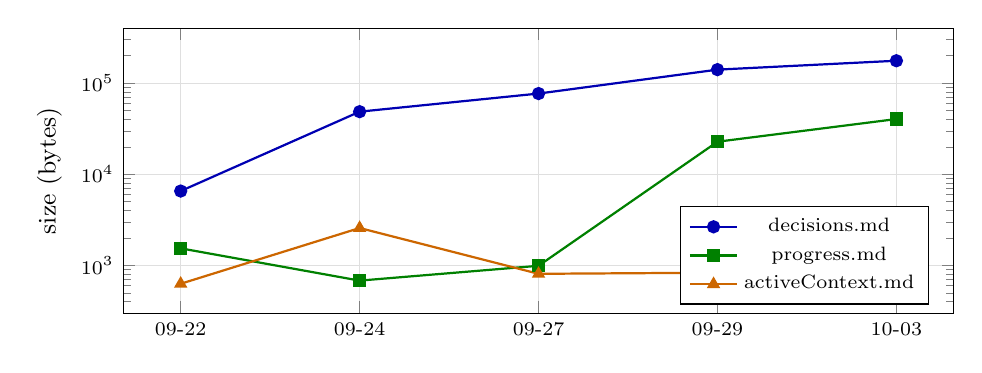
\begin{tikzpicture}
\begin{axis}[
  width=\columnwidth, height=5.2cm, ymode=log,
  symbolic x coords={09-22,09-24,09-27,09-29,10-03}, xtick=data,
  ylabel={size (bytes)}, legend pos=south east, legend style={font=\scriptsize},
  tick label style={font=\scriptsize}, label style={font=\small}, ymin=300, ymax=400000,
  enlarge x limits=0.08, grid=major, grid style={gray!25}]
\addplot[thick, mark=*, color=blue!70!black] coordinates {(09-22,6549)(09-24,48616)(09-27,76829)(09-29,140560)(10-03,175966)};
\addplot[thick, mark=square*, color=green!50!black] coordinates {(09-22,1541)(09-24,682)(09-27,992)(09-29,22761)(10-03,40358)};
\addplot[thick, mark=triangle*, color=orange!80!black] coordinates {(09-22,630)(09-24,2575)(09-27,810)(09-29,833)(10-03,887)};
\legend{decisions.md, progress.md, activeContext.md}
\end{axis}
\end{tikzpicture}
\caption{Size of the three main memory-bank files at sampled commits (log scale). The scratchpad stays flat, the decision log grows without bound, and \code{progress.md} drifted into a history.}
\label{fig:growth}
\end{figure}

\paragraph{The friction log.} Twenty-nine entries were written between 2026-09-29 and 2026-10-03, all now fixed. By area: webnav 12, codenav 8, shared MCP code 4, tooling 3, docs 2. By severity: confusing 15, wrong-result 8, blocked 3, missing-feature 2, slow 1. It is a small but complete bug tracker for the agent's own tools; one entry is the thread-bound SQLite failure of \jevmem{} itself (\S\ref{sec:eng}).

\paragraph{The \jevmem{} store.} The SpaceMaker database holds 79 notes in one scope (the largest id is 82: three notes were forgotten), of 189 characters on average (maximum 384; a decision-log entry averages about 1.4\,KB). They are linked by 657 edges (temporal 335, semantic 150, entity 143, causal 29) over 49 distinct entities. Three are pinned, three are superseded and the synthesis queue holds a resolved \emph{promote} proposal and six dismissed proposals of the (since removed) merge kind. All notes were created on 2026-10-03, while the facts they state are dated 2026-09-26 to 2026-10-02: the store was bootstrapped from the existing history, which also explains why the branch field is empty on every note.

\paragraph{A decision made because of a failure.} The decision of 2026-10-03, ``Three-way split between memory bank, \jevmem{} and \code{AGENTS.md}'', records its trigger: the store ``had picked up a copy of \code{activeContext.md}'s next steps and restatements of \code{AGENTS.md} rules''. We still find residue: note 1 is the tabs-indentation rule, explicitly marked as a hard rule in \code{AGENTS.md}, and note 10 restates the phase-gate rule. The decision was written to six places (instruction file, \code{memory/README.md}, the root README, two skills and \jevmem's README) and \emph{enforced in code} (status screen, instruction-file skip), which we regard as the more durable half.

\paragraph{Observed limits in the field.} (i) Every note has an empty branch field, so branch-aware ranking has done nothing here yet; a per-branch scope is the open item recorded in \code{activeContext.md}. (ii) The restatement filter misses some paraphrases (\S\ref{sec:eval}). (iii) The gap between the rule (``open items only'') and practice in \code{progress.md} shows that conventions without checks decay.

\section{Evaluation}
\label{sec:eval}

We evaluate retrieval, consolidation, the write and hook screens, and the vector index. Every number comes from the harness in the repository (\code{jevmem eval} and the scripts in \code{evals/}); a single live run per measurement; Jev is not perfectly deterministic, so differences under about 0.03 are noise. We do not re-measure \jevmempaper's LoCoMo question-answering accuracy: we measure whether the right \emph{note} reaches the agent, a different quantity.

\subsection{Datasets}

\begin{table*}[t]
\caption{Evaluation sets. ``Unans.'' = questions whose answer is not in memory (gold is empty).}
\label{tab:data}
\small
\begin{tabular}{@{}llll@{}}
\toprule
Set & Notes & Questions & Remark \\
\midrule
orbit & 25 & 30 (6 unans.) & in-sample tuning set \\
harbor & 40 & 41 (6 unans.) & held-out, run once with frozen defaults \\
LoCoMo c0--c9 & one per dialogue turn, sessions 1--4 & 45 (conv-26) + 272 (90 unans.) & adversarial questions with later evidence become unanswerable \\
SpaceMaker commits & 57 commit subjects & 31 (6 unans.) & private \\
srxy (commits + docs) & 138 & 47 (8 unans.) & private \\
\bottomrule
\end{tabular}
\end{table*}

The small sets were written by the author, the held-out set after the system existed, and most tuning data come from SpaceMaker. For LoCoMo~\cite{maharana2024locomo} we make one note per dialogue turn of sessions 1--4, stamped with the session date; adversarial questions whose evidence lies in later sessions become unanswerable. Metrics: \emph{recall} (fraction of gold notes returned), \emph{exact} (all gold notes returned), items and characters returned, latency, Jev calls and input tokens, and \emph{abstention} (\code{sufficient} is not true on an unanswerable question).

\subsection{Retrieval}

\begin{figure}[t]
\centering
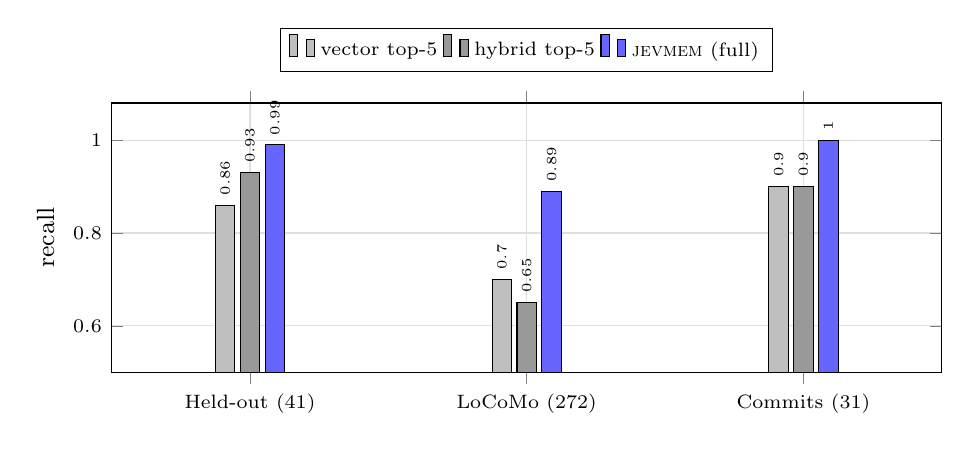
\begin{tikzpicture}
\begin{axis}[
  ybar, width=\columnwidth, height=5cm, bar width=7pt, ymin=0.5, ymax=1.08,
  symbolic x coords={Held-out (41),LoCoMo (272),Commits (31)}, xtick=data,
  ylabel={recall}, legend style={at={(0.5,1.28)},anchor=north,legend columns=-1,font=\scriptsize},
  tick label style={font=\scriptsize}, label style={font=\small}, enlarge x limits=0.25,
  nodes near coords, nodes near coords style={font=\tiny, rotate=90, anchor=west}, every node near coord/.append style={/pgf/number format/fixed, /pgf/number format/precision=2},
  grid=major, grid style={gray!25}]
\addplot[fill=gray!50] coordinates {(Held-out (41),0.86)(LoCoMo (272),0.70)(Commits (31),0.90)};
\addplot[fill=gray!80] coordinates {(Held-out (41),0.93)(LoCoMo (272),0.65)(Commits (31),0.90)};
\addplot[fill=blue!60] coordinates {(Held-out (41),0.99)(LoCoMo (272),0.89)(Commits (31),1.00)};
\legend{vector top-5, hybrid top-5, \jevmem{} (full)}
\end{axis}
\end{tikzpicture}
\caption{Recall of the gold note(s), \code{bge-small} embeddings. Baselines return five notes; \jevmem{} returns 1.4, 2.3 and 2.1 on average.}
\label{fig:recall-bars}
\end{figure}

Figure~\ref{fig:recall-bars} summarizes recall. On the held-out set \jevmem{} reaches 0.99 against 0.86 (vector) and 0.93 (hybrid); on pooled LoCoMo (9 conversations, 272 questions) 0.89 against 0.70 and 0.65; on SpaceMaker commit notes 1.00 against 0.90. Note that hybrid (BM25 $\oplus$ vector) is worse than vector on LoCoMo, where dialogue turns share vocabulary. At the same time \jevmem{} injects fewer notes: 1.4--2.3 instead of 5.

\begin{table}[h]
\caption{Pooled LoCoMo (272 questions), \code{bge-small}.}
\label{tab:locomo}
\small
\begin{tabular}{@{}lrrrrr@{}}
\toprule
Method & Recall & Items & Calls & Tokens & Latency \\
\midrule
vector top-5 & 0.70 & 5.0 & --- & --- & --- \\
hybrid top-5 & 0.65 & 5.0 & --- & --- & --- \\
lite & 0.84 & 3.0 & 1.0 & 2.1k & 0.25\,s \\
flat (no graph) & 0.85 & 1.6 & 4.0 & 3.8k & 0.94\,s \\
full & \textbf{0.89} & 2.3 & 5.9 & 9.5k & 1.44\,s \\
\bottomrule
\end{tabular}
\end{table}

\begin{table}[h]
\caption{Recall by question kind on pooled LoCoMo.}
\label{tab:kind}
\small
\begin{tabular}{@{}lrrrr@{}}
\toprule
Kind & $n$ & vector & lite & full \\
\midrule
single-hop & 102 & 0.70 & 0.87 & 0.92 \\
temporal & 48 & 0.81 & 0.90 & 0.94 \\
multi-hop & 19 & 0.60 & 0.76 & 0.82 \\
inference & 13 & 0.38 & 0.54 & 0.60 \\
\bottomrule
\end{tabular}
\end{table}

\paragraph{Where the graph helps.} On the single conversation conv-26, multi-hop recall rises from 0.20 (vector) to 0.70. On srxy, temporal questions score 0.04 (vector), 0.38 (lite) and 0.83 (full): the temporal graph and time-aware routing matter most for ``what did we decide \emph{before} X''. Honest counter-evidence: on srxy, graph expansion did not help (flat 0.93, full 0.92), and on pooled LoCoMo inference questions stay at 0.60.

\paragraph{Auto mode.} Pooled over 14 sets (466 questions), full reaches 0.910 recall at 10.4k tokens and 100\% escalation, lite 0.876 at 2.8k and 14\%, and the chosen \code{auto} setting (multi-hop $\ge 0.6$, temporal $\ge 0.8$) \textbf{0.911 at 6.3k tokens with 44\% escalation} (Figure~\ref{fig:tokens}). Dropping the temporal trigger cost srxy temporal recall (0.58 vs.\ 0.83); additionally escalating when lite says ``insufficient'' added 0.002 recall for 24\% more tokens and is off.

\begin{figure}[t]
\centering
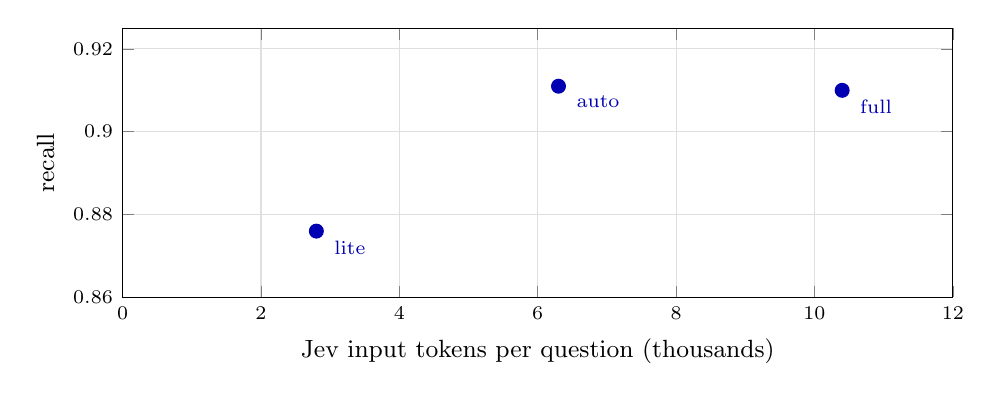
\begin{tikzpicture}
\begin{axis}[
  width=\columnwidth, height=5cm, xlabel={Jev input tokens per question (thousands)}, ylabel={recall},
  xmin=0, xmax=12, ymin=0.86, ymax=0.925, grid=major, grid style={gray!25},
  tick label style={font=\scriptsize}, label style={font=\small},
  nodes near coords, point meta=explicit symbolic, nodes near coords style={font=\scriptsize, anchor=north west, xshift=3pt}]
\addplot[only marks, mark=*, mark size=2.5pt, color=blue!70!black] coordinates {
 (2.8,0.876) [lite]
 (6.3,0.911) [auto]
 (10.4,0.910) [full]};
\end{axis}
\end{tikzpicture}
\caption{Cost--recall trade-off pooled over 14 sets (466 questions). Auto matches full recall for about 40\% fewer tokens.}
\label{fig:tokens}
\end{figure}

\subsection{Knowing what it does not know}

Because the agent is told to look elsewhere when memory is insufficient, abstention matters as much as recall. Full abstains on 85 of 90 unanswerable LoCoMo questions (94\%) and on all 6 of the SpaceMaker set; lite abstains on 94\% of 126 unanswerable questions pooled (97\% with the first thresholds, which flagged 11\% of answerable questions as insufficient; the chosen $0.3/0.7$ thresholds flag 4\%). The accuracy-optimal full-mode thresholds ($0.2$--$0.3/0.85$) score 0.89 against 0.85 for ours but let 9\% of unanswerable questions through instead of 5\%; leave-one-set-out accuracy is 0.88 either way, so we kept the defaults. The plain vector baselines can never abstain.

\subsection{Consolidation}

On labelled note pairs, each judged in both write orders (tuning 80 cases from 40 pairs, held-out 44 cases from 22 pairs): the original questions got 46/80 and 22/44 right; order-neutral questions got 79/80 and 43/44, and adding the ``reports a change'' question 80/80 and 44/44 with \textbf{no false flags on distinct pairs}. A fresh second held-out set (32 cases, 16 pairs) was 32/32. The new ``reports a change'' scores separate cleanly (superseded 0.68--0.97, others $\le 0.65$), as do coverage (duplicates $\ge 0.78$ both ways, subsumed $\ge 0.86$ one way, others $\le 0.42$) and pattern (repeated episodes 0.81--0.90, others $\le 0.59$). For same-timestamp ties, 32 of 36 became correctly superseded and all 18 true contradictions stayed \code{contradicts}. On SpaceMaker's live store, a full re-judge flagged exactly its three known stale notes (a fourth, a rename, later). The thresholds were tuned on the tuning set and checked on held-out sets; the pair sets are small.

\subsection{Write and hook screens}

\begin{table}[h]
\caption{Screens. ``Tune/holdout'' = threshold chosen on the first, checked on the second.}
\label{tab:screens}
\small
\begin{tabular}{@{}p{2.1cm}p{5.1cm}@{}}
\toprule
Screen & Result \\
\midrule
Injection & 0/15 benign blocked, 0/10 malicious missed (tuned on the same set: a regression test, not a rate) \\
Status ($\ge 0.85$) & 0 errors on tune (36) and holdout (24); status notes score $\ge 0.93$, others $\le 0.70$ \\
Auto-capture & 0 false captures on 123 real prompts (82 tune, 41 holdout); 11 of 12 synthetic standing rules stored \\
Prompt hook (needs-memory 0.20) & on-topic prompts with a gold note: 21/22; off-topic prompts with nothing injected: 19/22; 12/12 on the held-out prompts \\
Instruction-file skip & 19/23 restating notes by embedding alone; 22/23 with the borderline Jev band; 0 of 59 other notes skipped \\
\bottomrule
\end{tabular}
\end{table}

For SessionStart ranking over 31 sessions, hit@10 rises from 0.39 (no git context) to 0.52 (context weight 8). In a live session the instruction-file filter missed three paraphrases of a rule (coverage 0.30--0.43, below its threshold) while a non-restating note scored 0.49: no threshold separates them.

\subsection{Vector index}

At 100k notes (384-d, scoped top-10) the in-RAM matrix answers in 4.5\,ms (about 150\,MB), \code{sqlite-vec} in 12\,ms, LanceDB in 55--80\,ms. At one million notes (10 scopes, synthetic clustered vectors, 32 cores) the scoped p50 is 33\,ms for the matrix (1.5\,GB, exact), 44\,ms for \code{sqlite-vec}, 67\,ms for LanceDB IVF-PQ (recall 0.98), 3.5\,ms for a Qdrant server (0.996) and 3.3\,ms for pgvector HNSW with tuned parameters (0.975) but only 0.40 recall with defaults. A single developer's project stays far below 100k notes, so the default is exact search; the larger backends exist for shared stores.

\subsection{Threats to validity}

(1) \textbf{Small, author-written sets}: the held-out notes were written by the same person after the system existed. (2) \textbf{One run per measurement}; differences under 0.03 are noise. (3) \textbf{Tuning is dominated by SpaceMaker}; the hook and SessionStart weights come from 31 sessions and 44 prompts of one project. (4) \textbf{LoCoMo is conversational}; we convert turns to notes, which is not what our agents write. (5) \textbf{Unanswerable questions} are mostly adversarial in a style the model handles well. (6) \textbf{Vendor figures} (latency about 70--500\,ms per call, about \$0.042 per million input tokens) are quoted from the vendor and not independently measured. (7) The \textbf{field study} has one project, one developer and 12 days; it cannot show that the approach generalizes or measure the effect on agent task success.

\section{Discussion and Lessons}
\label{sec:discussion}

\paragraph{Separate by how knowledge ages, not by topic.} The most useful decision in the project was not an algorithm but a boundary: state, facts and rules age differently, so they need different stores and different update rules. A single semantic memory that accepts everything is easy to build and slowly poisons itself. We made the boundary mechanical where we could (a status screen at write time, an instruction-file filter at read time) and conventional where we could not (the ``both places'' rule for decisions). The conventions decayed: \code{progress.md} ignored its own size rule. We recommend checks, not prose.

\paragraph{What makes a good note.} The tool's constraints encode the lessons: \emph{one fact per note} (Jev judges literally and suffers context rot on long texts), an \emph{absolute date} (relative dates are rejected by auto-capture, and Jev cannot do date arithmetic), the \emph{entities by name}, and \emph{the reason in the same note} so that a recalled fact is actionable. Notes are data, not instructions: the hooks wrap them with a header saying so, and the injection screen guards the write path.

\paragraph{Typed judgments where decisions are bounded, an LLM where language is needed.} Every decision in the store has a bounded output and is cheap enough to run per write and per recall; code owns ordering, budgets and policy. The generative model is used where it is needed: writing the note, synthesizing a promoted pattern, answering. This split also made the system testable with a fake: a rule function replaces the model, and call counts become assertions. The cost is a dependency on a hosted, waitlisted model; the fail-closed/fail-open design limits the blast radius but does not remove it.

\paragraph{Supersede, do not delete.} Memory that is only appended turns contradictory; memory that is edited loses history. Marking older facts as superseded---ordered by code, not by the model---keeps the audit trail, keeps stale facts out of the context, and still lets the agent find ``what did we believe before''. The one place we had to leave a human-in-the-loop is conflicts the code cannot order, which become proposals.

\paragraph{Honesty about missing memory.} Returning \code{sufficient=false} instead of five nearest-but-irrelevant notes changes the agent's behaviour from guessing to looking. Abstention was the single most valuable property in daily use and the one that vector search cannot provide.

\paragraph{Limitations.} (i) Consolidation compares only the three nearest neighbours plus co-retrieved pairs, so a stale note that never surfaces next to its replacement is not caught. (ii) The status screen passes a status update phrased as a dated event. (iii) Auto-capture stores only 11/12 standing rules, by design. (iv) Squash-merged branches look abandoned. (v) Hook weights were tuned on one project. (vi) A note is only as trustworthy as its writers. (vii) The vendor model is hosted. (viii) Prompted sufficiency and escalation signals plateau at about 0.88 accuracy; a learned signal is future work. (ix) Our evaluation does not measure end-task success of an agent with and without the system.

\paragraph{Future work.} A per-branch scope; a re-run of the million-note benchmark with real embeddings and several writers; questions written by someone other than the system's author; hook-evaluation data from more than one store; a held-out split for the SessionStart weights; and a controlled study of agent task success with and without each tier.

\section{Conclusion}

Agent memory for software projects is not one problem. Current state, durable facts and standing rules age at different speeds and deserve different homes: git-tracked markdown, a typed note store, and the instruction file. The markdown memory bank carries the state; \jevmem{} carries the facts using a System-One/System-Two split in which a small typed model makes every high-frequency decision, code owns policy, and a generative model is never called inside the store. On our sets this retrieves better than vector search while injecting fewer notes and admitting when it does not know; on a real project it was used for twelve days alongside a memory bank that 78\% of commits touched. The most durable lesson came from a failure: when the semantic store started to hold the agent's next steps and the project's rules, the fix was a boundary, enforced in code. We hope the three-tier model and the open implementations are useful starting points.


\bibliographystyle{ACM-Reference-Format}
\bibliography{references}

\appendix
\section{Configuration Defaults}
\label{app:config}

\begin{table}[h]
\caption{Selected \code{Config} defaults (\code{jevmem 0.2.1}).}
\small
\begin{tabular}{@{}p{3.6cm}p{0.9cm}p{2.7cm}@{}}
\toprule
Parameter & Value & Role \\
\midrule
\code{relation_threshold} & 0.60 & edge stored \\
\code{write_candidates} & 10 & $K_w$ \\
\code{duplicate_similarity} & 0.97 & reject duplicate \\
\code{status_block} & 0.85 & reject status note \\
\code{injection_block} & 0.50 & reject injection \\
\code{capture_standing} & 0.70 & auto-capture \\
\code{recall_mode} & auto & lite then full \\
\code{lite_candidates} & 20 & vector top-$N$ \\
\code{lite_sufficient} & 0.30 & lite sufficient\\
\code{lite_missing_max} & 0.70 & lite missing\\
\code{escalate_multi_hop} & 0.60 & lite $\to$ full\\
\code{escalate_temporal} & 0.80 & lite $\to$ full\\
\code{activation_threshold} & 0.30 & graph active \\
\code{graph_budget}, \code{gamma} & 80, 1.0 & $B$, $\gamma$ \\
\code{anchor_count}, \code{rrf_k} & 30, 60 & anchors, $\kappa$ \\
\code{beam_width}, \code{max_depth} & 10, 8 & $W$, $D_{\max}$ \\
\code{sufficient} & 0.50 & stop rule $s_d$\\
\code{missing_max} & 0.60 & stop rule $m_d$\\
\code{contradiction_max} & 0.60 & stop rule $c_d$\\
\code{cont_threshold} & 0.15 & no expected gain \\
\code{max_nodes}/\code{max_edges} & 60/2400 & limits \\
\code{max_jev_calls}, \code{time_budget_s} & 19, 15 & limits \\
\code{top_k} & 8 & returned \\
\code{min_relevance} & 0.30 & drop anchors \\
\code{consolidate_every} & 20 & writes per pass \\
\code{consolidate_candidates} & 3 & neighbours \\
\code{conflict_same} & 0.70 & conflict\\
\code{conflict_different} & 0.85 & conflict\\
\code{conflict_outdated} & 0.80 & conflict\\
\code{conflict_change} & 0.80 & conflict\\
\code{cover_threshold} & 0.75 & duplicate/subsumed \\
\code{promote_threshold} & 0.75 & promote proposal \\
\code{hook_topic_min} & 0.60 & same-subject \\
\code{instructions_similarity} & 0.82 & restated filter\\
\code{instructions_band} & 0.70 & borderline band\\
\code{session_context_weight} & 8.0 & git boost \\
\code{unmerged_penalty} & 0.8 & other-branch notes \\
\code{superseded_penalty} & 0.6 & stale notes \\
\bottomrule
\end{tabular}
\end{table}

\section{MCP Tools}
\begin{itemize}\small
\item \code{memory_write(content, scope, entities, timestamp, source, pinned)} $\to$ id, rejection reason, degraded flag, top types, edges, consolidation report.
\item \code{memory_recall(query, scope, max_items, mode)} $\to$ evidence (id, content, timestamp, scope, score, flags), \code{sufficient}, \code{missing}, \code{stop_reason}, \code{jev_calls}, \code{hint}.
\item \code{memory_pin}, \code{memory_list}, \code{memory_forget}, \code{memory_stats}.
\item \code{memory_consolidate(all_notes)}, \code{memory_pending_synthesis}, \code{memory_resolve(synthesis_id, text)}, \code{memory_dismiss}, \code{memory_flush_pending}.
\end{itemize}

\section{Memory-Bank Templates}
\begin{verbatim}
## YYYY-MM-DD: <title>        (decisions.md)
Context: ...   Decision: ...   Rationale: ...

# Active context             (activeContext.md)
Branch / Current focus / Blockers /
Just changed / Next steps

date, area, severity, status  (friction/*.md)
Call / Expected / Got / Workaround / Idea
\end{verbatim}

\section{Question Style}
Jev questions are plain English over a named-JSON state. Two representative ones (paraphrased from \code{questions.py}): the \emph{status} question for a write (``Does this observation describe the current state of ongoing work---what is happening now or what to do next---rather than a lasting fact?'') and the order-neutral \emph{reports-change} question for consolidation (``Does either text report that what the other says has changed?'', asked in both directions, maximum taken).


\end{document}
